\documentclass[11pt]{article}
\usepackage[margin=1in]{geometry}
\usepackage{amsmath,amssymb}
\usepackage{graphicx}
\usepackage{booktabs}
\usepackage[colorlinks=true,linkcolor=blue,citecolor=blue,urlcolor=blue]{hyperref}

% --- the only two lines to edit before submission ---
\newcommand{\authorname}{Singularity}
\newcommand{\affiliation}{}

\title{Are cognitive subtypes real? Null-calibrated consensus clustering\\ for test batteries: a simulation study}
\author{\authorname\\ \small \affiliation}
\date{\today}

\begin{document}
\maketitle

\begin{abstract}
Subtyping studies in cognitive and clinical psychology cluster test scores and report profiles. Most cognitive
batteries, however, share one general factor, and many scores are skewed or have ceiling effects. We ask how often
four procedures report subtypes in simulated batteries (300 participants, 8 tests) that have none, and how often they
find subtypes that are there: $k$-means with a silhouette threshold, latent profile analysis (diagonal Gaussian
mixtures chosen by BIC), full-covariance Gaussian mixtures chosen by BIC, and consensus clustering calibrated against a
correlation-preserving null --- an approach developed in cancer genomics and, to our knowledge, not used in psychology.
Latent profile analysis reported subtypes in 100\% of datasets, with or without real subtypes. Full-covariance
mixtures reported subtypes in 100\% of skewed or ceiling-limited null datasets and in none of the datasets with real
subtypes. $k$-means reported false subtypes in 45--55\% of non-normal null datasets and found real ones in at most
20\%. Calibrated consensus clustering was the only procedure whose rate differed between the two situations: 15--30\%
false discoveries (above its nominal 9\%) and 30--95\% detection, increasing with separation. The common practice of
choosing the number of latent profiles by BIC cannot, in this setting, tell subtypes from a single continuous ability.
\end{abstract}

\section{Introduction}
Data-driven subtyping is widespread in psychology and psychiatry: cognitive profiles in ADHD, autism or ageing, or
clinical subtypes of depression. Latent profile analysis (LPA) with information criteria is the most common tool.
Two features of cognitive data make it fragile. First, tests correlate through a general factor, which violates the
local independence assumed by diagonal mixtures~\cite{BauerCurran}. Second, scores are often skewed or capped, and
mixture models fit non-normality with extra components~\cite{BauerCurran}. In genomics, consensus
clustering~\cite{Monti} was found to produce structure in null data~\cite{Senbabaoglu}, which led to calibrating it
against simulated nulls that keep the correlation structure of the data (M3C~\cite{John}). We transfer this
calibration to test batteries and compare it with the usual procedures, on data where the truth is known. The question
was prompted by an automated forecast that consensus clustering would enter experimental and cognitive psychology.

\section{Methods}
\paragraph{Data.} 300 participants, 8 standardised tests, one factor with loading 0.6. Null scenarios: normal
scores; four tests skewed ($e^{0.8x}$); four tests with a ceiling at $+0.5$ SD. Subtype scenarios: two or three
equal-sized subtypes, each stronger by $d$ SD on a different block of three tests, $d\in\{1.0,1.5,2.0\}$, on top of the
same factor structure. 40 datasets per scenario.
\paragraph{Procedures} (each declares ``subtypes'' or not).
\begin{itemize}
\item $k$-means, best $k\in\{2,\dots,5\}$ by silhouette; subtypes if the silhouette exceeds 0.25.
\item LPA: diagonal Gaussian mixtures, $k\in\{1,\dots,5\}$ by BIC; subtypes if $k>1$.
\item Full-covariance Gaussian mixtures, same rule.
\item Consensus clustering: $k$-means on 25 subsamples of 80\%, proportion of ambiguous clustering (PAC) for each
$k$; 10 null datasets drawn from a multivariate normal with the observed covariance; subtypes if, at the $k$ with the
largest gap, the observed PAC is below all 10 null values (nominal level $1/11\approx9\%$).
\end{itemize}
All settings and the seed were fixed before the single run.

\section{Results}
\begin{figure}[t]
\centering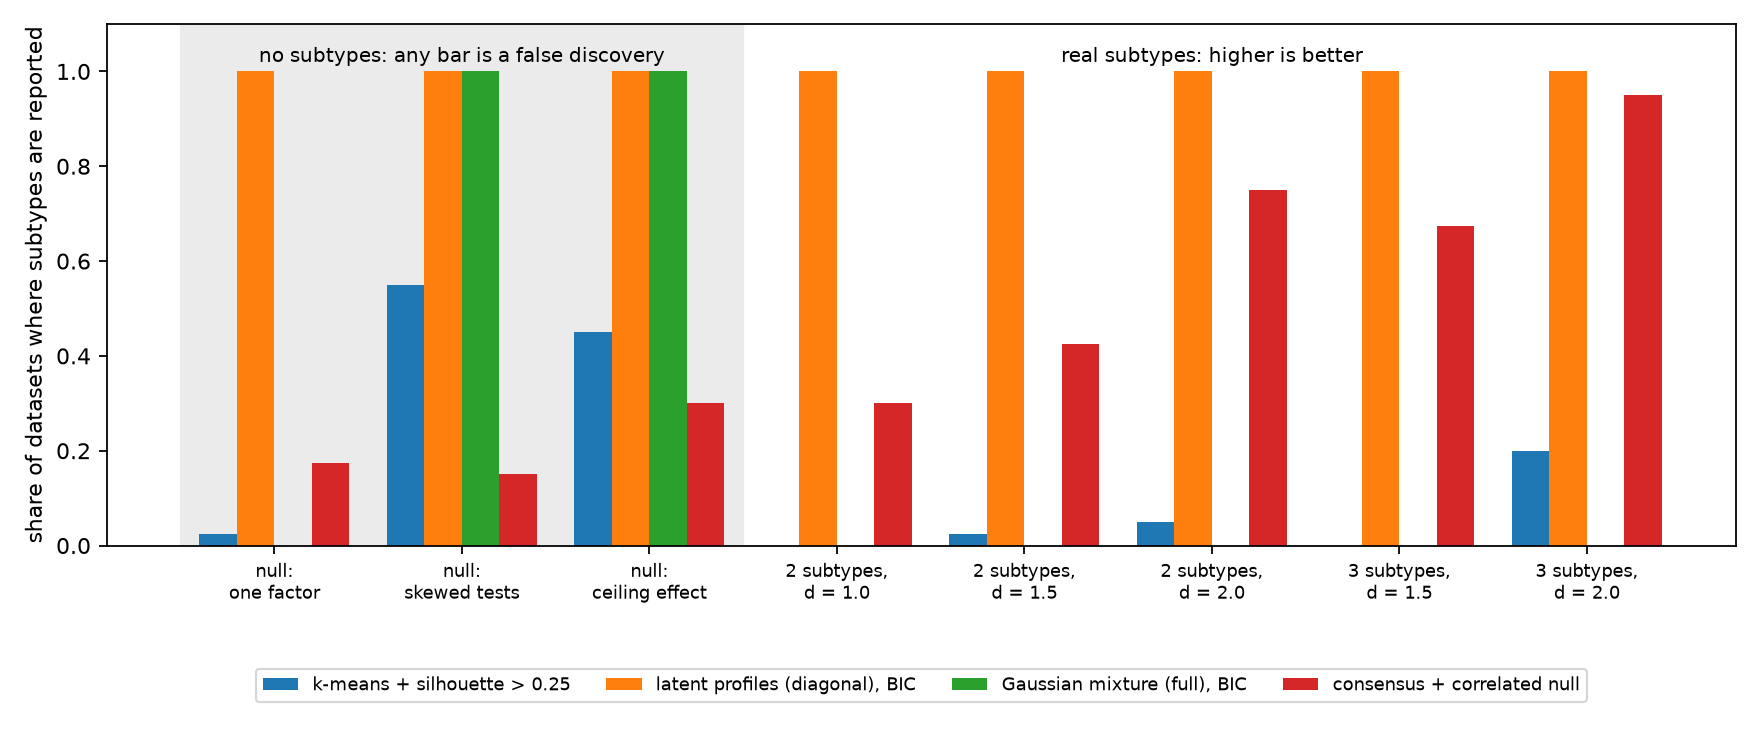
\includegraphics[width=\linewidth]{fig_rates.png}
\caption{Share of datasets in which each procedure reports subtypes.}
\label{fig}
\end{figure}

\begin{table}[h]
\centering
\begin{tabular}{lccc|ccccc}
\toprule
 & \multicolumn{3}{c|}{no subtypes} & \multicolumn{5}{c}{real subtypes} \\
procedure & normal & skewed & ceiling & 2, d=1 & 2, d=1.5 & 2, d=2 & 3, d=1.5 & 3, d=2 \\
\midrule
$k$-means + silhouette & 0.03 & 0.55 & 0.45 & 0.00 & 0.03 & 0.05 & 0.00 & 0.20 \\
LPA (diagonal), BIC & 1.00 & 1.00 & 1.00 & 1.00 & 1.00 & 1.00 & 1.00 & 1.00 \\
full mixture, BIC & 0.00 & 1.00 & 1.00 & 0.00 & 0.00 & 0.00 & 0.00 & 0.00 \\
consensus + correlated null & 0.18 & 0.15 & 0.30 & 0.30 & 0.43 & 0.75 & 0.68 & 0.95 \\
\bottomrule
\end{tabular}
\caption{Share of 40 datasets in which subtypes are reported.}
\label{tab}
\end{table}

Table~\ref{tab} and Figure~\ref{fig} show three failures and one partial success.
\begin{itemize}
\item \textbf{LPA always finds profiles.} Because the tests correlate, a diagonal mixture needs several components
to reproduce a single factor; BIC prefers them every time.
\item \textbf{Full mixtures confuse shape with subtypes.} They handle the correlation, but fit skew and ceilings with
extra components, and in our subtype scenarios the extra component never paid its BIC penalty.
\item \textbf{$k$-means with a silhouette rule} is driven by marginal shape more than by groups.
\item \textbf{Calibrated consensus clustering separates the two situations}, with detection growing with separation,
but its false-discovery rate (15--30\%) exceeds the nominal 9\% because the normal null does not reproduce skew and
ceilings.
\end{itemize}

\section{Discussion}
In cognitive batteries with one general factor, a reported number of latent profiles chosen by BIC carries little
information about whether subtypes exist. Calibrating consensus clustering against a null that keeps the observed
correlations is a better default, and should be extended with nulls that also keep the marginal distributions (for
example a Gaussian copula of the observed margins), which would address the excess false discoveries we observed.

\paragraph{Limitations.} One factor structure, one sample size, equal subtype sizes, 10 null references; no
real data.

\paragraph{Reproducibility.} \texttt{experiment.py} regenerates every number and the figure.

\paragraph{Origin of the question.} The question came from an automated forecast (Singularity v3, registered on 5
November 2026 with a SHA-256 fingerprint) that consensus clustering would enter the subfield \emph{Experimental and
Cognitive Psychology}. The forecast concerned the arrival of the method, not the result of this study.

\begin{thebibliography}{9}
\bibitem{BauerCurran} D.~J.~Bauer, P.~J.~Curran, Distributional assumptions of growth mixture models: implications for
overextraction of latent trajectory classes, \emph{Psychological Methods} 8 (2003) 338--363.
\bibitem{Monti} S.~Monti et al., Consensus clustering, \emph{Machine Learning} 52 (2003) 91--118.
\bibitem{Senbabaoglu} Y.~\c{S}enbabao\u{g}lu, G.~Michailidis, J.~Z.~Li, Critical limitations of consensus clustering in
class discovery, \emph{Scientific Reports} 4 (2014) 6207.
\bibitem{John} C.~R.~John et al., M3C: Monte Carlo reference-based consensus clustering, \emph{Scientific Reports} 10
(2020) 1816.
\end{thebibliography}
\end{document}
